%!TEX root = causalityRetweetPropensity.tex
\section{Diego Section}
\subsection{Motivation}
In the third experiment we attempted to see if we could observe network effects in the dataset. It is well known that network effects can have a significant impact on the behavior of its members[Easley].  In particular we searched for evidence of “Latent Homophily” and “Social Contagion” in the Tweeter message network of a very well know political figure in Latin American.  Latent Homophily is the tendency for the members of a social network to share similar characteristics because a “latent” characteristics lead the individual to join the social network in the first place[Shalizi].  Social Contagion is the tendency for the members of a social network to share similar characteristics because of direct influence between the member of the social network [Shalizi].

Although [Shalizi] showed that separating the Latent Homophily and Social Contagion is very difficult, we hypothesized that we could observe evidence of either or both by measuring the number of mentions an individual makes.  Mentions are direct references to an individual or group in Tweeter.  We hypothesized that the strength of membership on an individual belonging to a social group could be estimated by counting the number of mentions that individual makes about the organization.  Similarly, we hypothesized that the level of influence on an individual by other members of the social group could be estimated by counting the number of times an individual is mentioned by others.  We developed a Probabilistic Soft Logic (PSL) predictive model to attempt to predict the propensity of an individual to retweet based on the number of mentions that individual received and made.

\subsection{Data}
This experiment was run on a subset of the dataset described above.  In particular, we used all Tweets associated with Nicolas Maduro, the president of Venezuela.  These include all tweets by Nicolas Maduro, all tweets that mention Nicolas Maduro, and all retweets of postings made by him.  Nicolas Maduro is a well known and very polemic individual in Latin American.  The training set consisted of 179 tweets that originated from the Nicolas Maduro account; 89,303 retweets of the original tweets; and 288,564 tweets that mentioned Nicolas Maduro (excluding retweets).  The test set contained 87 tweets that originated from the Nicolas Maduro account;  13,281 retweets of the original tweets; and 97,901 tweets that mentioned Nicolas Maduro (excluding retweets).  The train and test sets do not overlap in time.

\subsection{Methods}
The PSL program described in the introduction contained the following rules:

1. Estimating Homophily Strength: The higher the number of “Organization” mentions by an “Individual A” implies a higher propensity for “Individual A” to retweet messages posted by the “Organization”. 

m.add rule : ( PostedInd(U,M) & HasGroupMention(M,G) ) >> RetweetedGroup(U),  weight : 1

Where:
U is an individual
G is the group
M is the tweet

2. Estimating Contagion: The higher the number of mentions received by an “Individual A” implies a higher propensity for “Individual A” to retweet messages posted by the “Organization”.  “Individual A” has been identified (outside of PSL) as belonging to the social network associated with the “Organization”.  Versions of this rule include adjustments for the sentiment of the tweets.

m.add rule : ( PostedInd(U1,M) & Mentions(M,U2) ) >> RetweetedGroup(U2),  weight : 1
m.add rule : ( PostedInd(U1,M) & Mentions(M,U2) & Positive(M) ) >> RetweetedGroup(U2),  weight : 1
m.add rule : ( PostedInd(U1,M) & Mentions(M,U2) & Negative(M) ) >> ~RetweetedGroup(U2),  weight : 1

Where:
U1 and U2 are individuals
G is the group
M is the tweet

A graphical interpretation of the rules can be observed in Figure XX.  
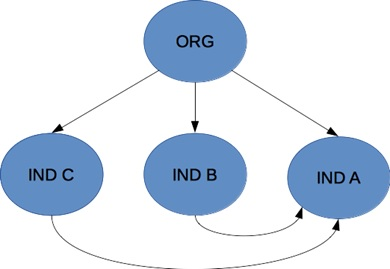
\includegraphics[100,100]{PSL_model.jpeg}

The propensity to retweet in the training set was calculated following the procedure below:

1. Take the average and standard deviation of the counts of retweets made by each individual.
2. Make the measure linear by taking 0 as no evidence observed and 1 for evidence equal or higher than the mean plus two standard deviations as determined in 1.

The training set was used to train (compute weights) the PSL model.  The learned model was then used to predict the propensity of an individual to retweet in the test set.

We run two sub-experiments on the data.  In the first one, we discretized the propensity to retweet by dividing the values into three groups (low, medium, and high propensity to retweet scores), each having the same number of members.  The mid value in each range was used as the retweet propensity for the entire group.  In the second sub-experiment, the propensity to retweet values without adjustments were used.

\subsection{Results}
Figure 2 and 3 shows the results of the observational study performed on the discretized and non-discretized propensity scores respectively. It displays the actual and predicted propensity to retweet calculated as described in the previous section.   The effect are small as suggested by the slop of the best fit lines, but the effect are statistically significant with p values of 2.2e-16 in both cases.  The low R-squared values indicate the model fits the data poorly as expected.  

The probability of an individual to retweet a message from an organization is very difficult to predict because it is the result of a very complex process involving several factors, many of which are latent.  The complete understanding of the process probably involves factors related to the Organization such as its political stance, popularity and the strength of its following.  Factor related to the message are most likely very important, such us the topic (or how interesting the topic is to the intended audience), the language used (funny, motivating, informative).  Factors related to the receiver such as its propensity to retweet, gender, age, culture and individual interests are all also likely very important.  
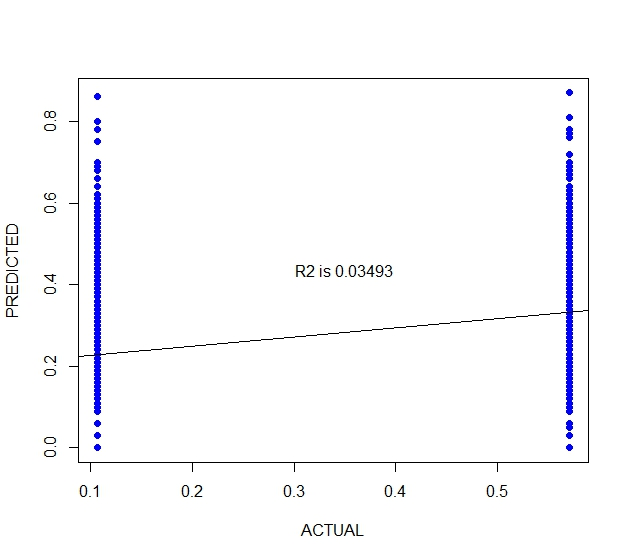
\includegraphics[100,100]{PredictedvActual_binning.jpeg}
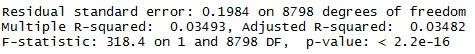
\includegraphics[100,100]{R2_results_binning.jpeg}
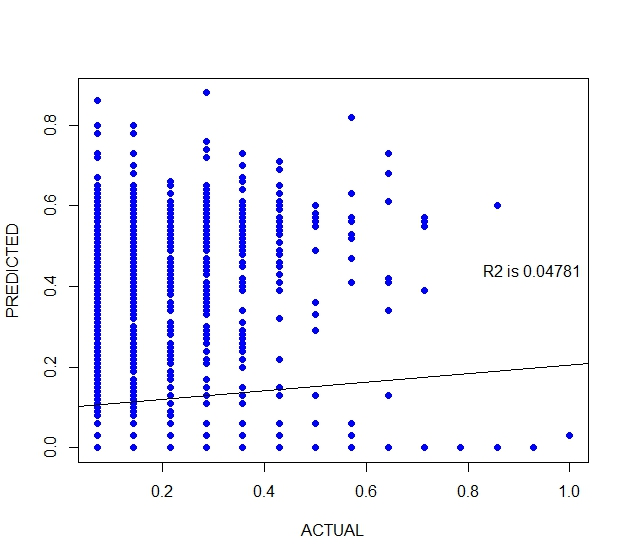
\includegraphics[100,100]{PredictedvActual.jpeg}
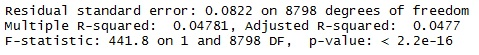
\includegraphics[100,100]{R2_results.jpeg}
